% Author: Carles Marin (Claude, Anthropic, as AI research assistant).
% Part IV. The second inversion-fixed point: a closed form for the Schur function at the generic
% element of the non-identity component of O(2n), of which Part III's class is the zero
% locus. Question-threaded narrative; honest about scope throughout. Build: pdflatex x2.
\documentclass[11pt,a4paper]{article}
\usepackage[utf8]{inputenc}
\usepackage{amsmath,amssymb,amsthm}
\usepackage{booktabs}
\usepackage[table,dvipsnames]{xcolor}
\usepackage{graphicx}
\usepackage{tikz}
\usetikzlibrary{shapes.geometric,arrows.meta,positioning,fit,backgrounds,patterns,calc}
\usepackage{geometry}
\geometry{margin=2.4cm}
\usepackage[colorlinks=true,linkcolor=RoyalBlue,citecolor=BrickRed,urlcolor=RoyalBlue]{hyperref}
\usepackage{caption}
\captionsetup{font=small,labelfont=bf}
\newtheorem{theorem}{Theorem}
\newtheorem{lemma}{Lemma}
\newtheorem{corollary}{Corollary}
\newtheorem{proposition}{Proposition}
\newtheorem{observation}{Observation}
\newcommand{\ZZ}{\mathbb{Z}}
\newcommand{\RR}{\mathbb{R}}
\newcommand{\su}[1]{SU(#1)}
\newcommand{\lam}{|\lambda|}
\definecolor{okgreen}{RGB}{0,140,54}
\definecolor{hdrblue}{RGB}{31,78,121}
\definecolor{softgrey}{RGB}{238,242,247}
\definecolor{warmred}{RGB}{178,34,34}

\title{\textbf{\Large Schur Functions at $(1,-1,t,t^{-1})$}\\[7pt]
\large\textnormal{\itshape A closed form on the non-identity component of $O(4)$:\\
three $SU(2)$ characters read off the $2$-quotient}\\[8pt]
\normalsize\textnormal{Part IV --- a vanishing criterion with no hypothesis on the shape of
the partition, the row that is not constant, and an open problem its owners declared}}
\author{Carles Mar\'in\thanks{Independent researcher, \texttt{karlesmarin@gmail.com}.
The computations were carried out and cross-checked with Claude (Anthropic) as an AI
research assistant against a common machine-verifiable ground truth (exact integer Laurent
arithmetic in SageMath, with every identity re-derived by a second, independent
implementation); every number in this paper regenerates from the ancillary scripts.}}
\date{\today}

\begin{document}
\maketitle

\begin{abstract}
\noindent
Part~III left one item open and said so: whether its classification of the representations
whose character vanishes identically on the non-identity component of $O(4)$ was a corollary of
some general criterion. It is --- and of something stronger than a criterion. For every
partition $\lambda$ with at most four rows,
$s_\lambda(1,-1,t,t^{-1})$ is $\pm$ a product of \emph{exactly three} $SU(2)$ characters, read
off the $2$-quotient of $\lambda$, or zero, with no hypothesis whatever on the shape of
$\lambda$; the vanishing classification is precisely its zero locus. The consequence is a
compression: conditionally on this identity, an arbitrarily large four-row partition collapses
to three integers with no loss of anything the physics of Part~III can see, so that every
quantity surviving its leading cancellation factors through the $2$-quotient and weight
enumeration is replaced by explicit polynomial formulae. The alphabet
$\{1,-1,t,t^{-1}\}$ is the generic semisimple element of $O(4)^-$, and it sits between two
factorisation programmes and belongs to neither: the reciprocal-pair line of
Ciucu--Krattenthaler and Ayyer--Behrend, whose engine needs every inversion-fixed point of the
alphabet to contribute a \emph{constant} row of the bialternant --- which $+1$ does and $-1$
does not --- and the root-of-unity line of Littlewood, Prasad, Ayyer--Kumari and Karmakar,
whose alphabets carry a free variable in every letter. Replacing the two fixed-point rows by
even/odd column indicators repairs the argument at rank one and does not at rank two, which is
where we stop and say so. We state the identity as \emph{verified} and not as a theorem: it is
checked exhaustively by two independent implementations on all $3060$ partitions with four
parts $\le14$ and all $4845$ with parts $\le16$, with no mismatch and no residue in the zero
locus, and no proof is given. Ciucu--Krattenthaler wrote in 2008 that they could not offer a
representation-theoretic interpretation of their factorisations, and Ayyer--Behrend and
Ayyer--Kumari repeated it in 2018 and 2025; the reading offered here --- a character on the
non-identity component --- is of that kind, conditional on the identity being true, and it
reaches the factorisation and not only the vanishing. \emph{Added in version~3:} that reading has a
home in the literature we failed to cite in version~1. Characters of a disconnected group on a
non-identity component are \emph{twining characters}, and the identity that computes them by folding
is due to Jantzen~\cite{Jantzen} and, in the form closest to ours, to Kumar--Lusztig--Prasad~\cite{KLP};
our restriction is reducible, so it is reached from theirs by one step of Clifford theory. The
mechanism is theirs and we credit it here; what this paper contributes is the explicit evaluation at
free~$t$. What we take to be the result of this
paper, however, is neither the identity nor that reading, but what they make possible:
$\Phi=F\circ Q$, the physical functional factoring through the $2$-quotient. The Schur identity
is the door; the reduction is what is behind it.
\end{abstract}

% ===================================================================
\section{The item we left open}\label{sec:intro}

Part~III classified, in $\su4$ Dynkin labels, the representations for which
\begin{equation}\label{eq:D}
D(t)\;=\;s_\lambda(1,-1,t,t^{-1})
\end{equation}
vanishes identically. The classification was exact, it was certified in Lean, and it was
honest about what it owed: the \emph{mechanism} is classical --- an $O(2n)$ irreducible
representation and its associate $\mu\otimes\det$ have opposite characters on the
non-identity component (the \emph{improper} component, in the older terminology), so self-associate ones contribute nothing there --- and what was claimed was the
arithmetic, not the phenomenon. That paper ends by stating four questions it cannot answer.
We quote them verbatim from its version~5~\cite{PartIII}, resolving in brackets the two
cross-references that are internal to it:

\begin{quote}
\textbf{Q1} Is $\mathcal Z$ a corollary of some general criterion for a $GL(n)$ character
to vanish on the non-identity component, or is it particular to $\su4$?\quad
\textbf{Q2} The theorem says where $D$ is zero. \emph{What is $D$ when it is not?} We use
its coefficients throughout and never learn what function they belong to.\quad
\textbf{Q3} Why exactly two branches? [Part~III, Figure~6] shows no third cause of
vanishing, and we have no reason why there could not be one.\quad
\textbf{Q4} The moments $\sum_m m^{2r}\delta(m)$ decide everything that survives
[Part~III, \S6], and we obtain them by enumerating the weight system of each irreducible.
Is there structure there, or is enumeration the only route?
\end{quote}

The four have one answer between them, and it is the subject of this paper:
\begin{center}\small
\begin{tabular}{ll}
\toprule
\rowcolor{hdrblue}\textcolor{white}{question} & \textcolor{white}{answer, and where}\\
\midrule
\textbf{Q1} general criterion? &
yes, and by something stronger --- \S\ref{sec:closedform}\\
\rowcolor{softgrey}
\textbf{Q2} what is $D$ when non-zero? &
$\pm$ three $SU(2)$ characters off the $2$-quotient --- \eqref{eq:closedform}\\
\textbf{Q3} why exactly two branches? &
a product of three characters has exactly two ways to vanish --- \S\ref{sec:zero}\\
\rowcolor{softgrey}
\textbf{Q4} structure in the moments? &
$\delta$ is a threefold convolution; every moment is polynomial --- \S\ref{sec:moments}\\
\bottomrule
\end{tabular}
\end{center}

This paper answers it. The answer is not a criterion. It is a closed form for the character
itself, of which the criterion is the locus where the form evaluates to zero.

One word about priority among the four, because it shapes everything after \S\ref{sec:zero}.
\textbf{Q1}--\textbf{Q3} are about the zeros, and the zeros were already classified: Part~III
proves that outright. \textbf{Q4} is about what is left once the leading term has cancelled,
and that was the question Part~III actually needed answered and could not. So the centre of
this paper is not the vanishing criterion but \eqref{eq:factorfunctional} in
\S\ref{sec:moments}: the physical functional factors through the $2$-quotient. The closed form
is how that becomes possible; it is the mechanism, not the point (Figure~\ref{fig:chain}).

\begin{figure}[h]
\centering
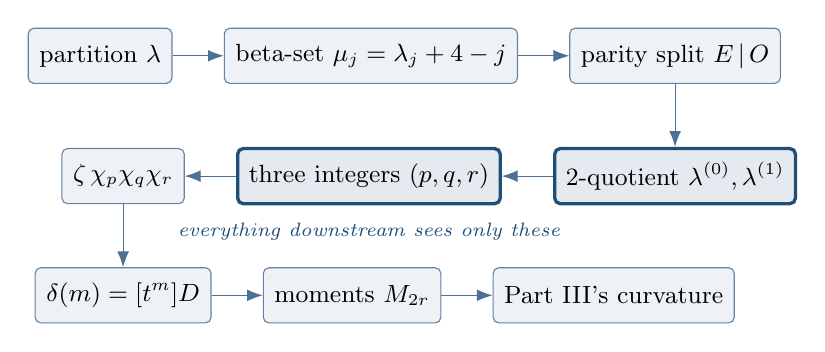
\begin{tikzpicture}[node distance=6.5mm,
  every node/.style={font=\small},
  box/.style={draw=hdrblue!70,fill=softgrey,rounded corners=2pt,inner sep=4pt,minimum height=7mm},
  ours/.style={draw=hdrblue,fill=hdrblue!12,rounded corners=2pt,inner sep=4pt,
               minimum height=7mm,very thick},
  ar/.style={-{Latex[length=2mm]},draw=hdrblue!80}]
\node[box] (l) {partition $\lambda$};
\node[box,right=of l] (mu) {beta-set $\mu_j=\lambda_j+4-j$};
\node[box,right=of mu] (par) {parity split $E\,|\,O$};
\node[ours,below=8mm of par] (quo) {$2$-quotient $\lambda^{(0)},\lambda^{(1)}$};
\node[ours,left=of quo] (pqr) {three integers $(p,q,r)$};
\node[box,left=of pqr] (chi) {$\zeta\,\chi_p\chi_q\chi_r$};
\node[box,below=8mm of chi] (d) {$\delta(m)=[t^m]D$};
\node[box,right=of d] (mom) {moments $M_{2r}$};
\node[box,right=of mom] (phys) {Part~III's curvature};
\draw[ar] (l)--(mu); \draw[ar] (mu)--(par); \draw[ar] (par)--(quo);
\draw[ar] (quo)--(pqr); \draw[ar] (pqr)--(chi); \draw[ar] (chi)--(d);
\draw[ar] (d)--(mom); \draw[ar] (mom)--(phys);
\node[below=1mm of pqr,font=\scriptsize\itshape,text=hdrblue] {everything downstream sees only these};
\end{tikzpicture}
\caption{The chain, and where it narrows. Reading left to right and then back, a partition with
four rows --- of unbounded size --- is compressed at the third step into three integers, and
nothing downstream ever sees anything else. The two boxed steps are what this paper supplies;
the rest is standard. \eqref{eq:factorfunctional} states the narrowing as an identity of
functionals.}
\label{fig:chain}
\end{figure}

These two papers should be read as a pair, and the pairing is not merely editorial. Part~III is
a physics argument that ran into a question about symmetric functions and exported it; this one
answers that question and hands back a tool the physics needed and did not have. The exchange
closes in \S\ref{sec:moments}: the same factorisation that decides where the character vanishes
also makes every moment of its coefficient sequence a polynomial in three integers, and those
moments are what Part~III was obtaining by enumerating weight systems. A reader interested only
in the combinatorics may stop before that section; a reader who came from Part~III should start
there.

The object is not exotic. Since $1\cdot(-1)\cdot t\cdot t^{-1}=-1$ and the multiset is stable
under $x\mapsto x^{-1}$, the alphabet $\{1,-1,t,t^{-1}\}$ is the eigenvalue multiset of an
element of $O(4)$ with $\det=-1$: the generic semisimple element of the non-identity
component. So \eqref{eq:D} is a $GL(4)$ character restricted to the non-identity component, and the
question ``when does it vanish, and what is it when it does not'' is a question about
characters on a disconnected group. That framing is what made the search tractable, and it is
also what explains why the answer was not already on the shelf.

% ===================================================================
\section{Two programmes, and the gap between them}\label{sec:gap}

Specialisations of Schur functions that factorise are a subject with two active lines, and our
alphabet falls between them.

\paragraph{The reciprocal-pair line.} Ciucu--Krattenthaler~\cite{CK} and then
Ayyer--Behrend~\cite{AB} factorise $s_\lambda$ at
\begin{equation}\label{eq:ABalphabets}
(X,\bar X),\qquad (X,\bar X,1),\qquad (X,\bar X',1),
\end{equation}
into products of orthogonal and symplectic characters, for $\lambda$ self-complementary in a
rectangle. Their engine is a single block identity, Ayyer--Behrend Eq.~(23):
\begin{equation}\label{eq:blockid}
\det\begin{pmatrix}A&B\\B&A\end{pmatrix}
=\det\begin{pmatrix}A-B&B\\B-A&A\end{pmatrix}
=\det\begin{pmatrix}A-B&B\\0&A+B\end{pmatrix}
=\det(A-B)\,\det(A+B),
\end{equation}
reached by scaling rows to remove the rectangle width and reversing the columns of the right
block so that the two exponent multisets coincide. The self-complementary hypothesis is
consumed \emph{only} in that column reversal, and it says exactly one thing: the beta-set is
symmetric about its midpoint.

\paragraph{The root-of-unity line.} Littlewood~\cite{LittlewoodBook}, Prasad~\cite{Prasad}, Ayyer--Kumari~\cite{AK},
Kumari~\cite{Kumari}, Albion~\cite{Albion} and Karmakar~\cite{Karmakar} work at
$(X,\omega X,\dots,\omega^{t-1}X)$ and its variants, where the vanishing is governed by the
$t$-core of $\lambda$ and the factorisation by the $t$-quotient.

\paragraph{Ours is in neither.} $\{1,-1\}\cup\{t,t^{-1}\}$ is not of the form $(X,\bar X)$:
solving $\{t,t^{-1}\}=\{y,-y\}$ forces $t^2=-1$, so $t$ is not free. And it is not
$\omega^kX$: the letters $\pm1$ carry no free variable. The natural place for it in
\eqref{eq:ABalphabets} is the next member of the sequence,
\begin{equation}
(X,\bar X,1,-1),
\end{equation}
the case in which \emph{both} fixed points of $x\mapsto x^{-1}$ are present rather than one.
That member is missing (Figure~\ref{fig:families}), and the reason is sharper than an oversight, as \S\ref{sec:why} shows.

\paragraph{Open flank.} Why are these two programmes separate at all? Both compute
specialisations at elements of a classical group; one takes the element to have distinct
reciprocal eigenvalue pairs, the other to have eigenvalues on a $\mu_t$-orbit. A general
alphabet is a multiset of roots of unity times monomials in free moduli, and the two programmes
are the two extreme cases of that. \emph{Is there a classification of which such
specialisations factorise?} We do not know of one, and the obvious conjecture --- that
factorisation is controlled by how the element's centraliser sits inside the group --- is easy
to state and, on the evidence of \S\ref{sec:ranktwo}, not obviously true.

\begin{figure}[h]
\centering
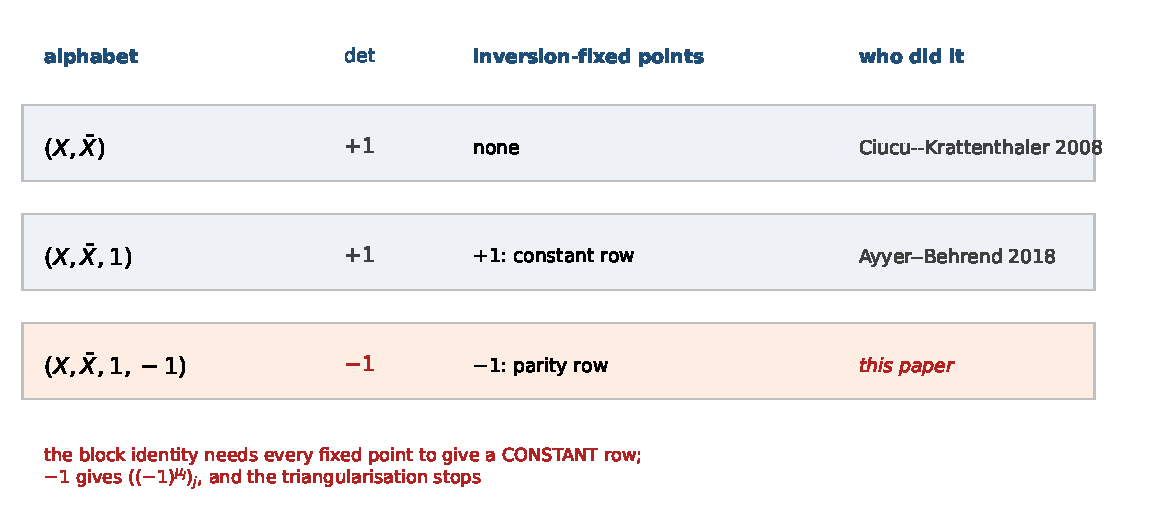
\includegraphics[width=0.94\textwidth]{fig_families.pdf}
\caption{The sequence, and the step that was never taken. Each row is an alphabet stable under
$x\mapsto x^{-1}$; the third column counts the points that stability leaves fixed, because
those are the ones that contribute a row to the bialternant on their own. Adding the first
fixed point $+1$ costs nothing --- its row is constant, and the block argument absorbs it.
Adding the second changes the determinant of the element from $+1$ to $-1$, i.e.\ moves it off
the identity component, and its row is a parity character rather than a constant. Everything in
this paper is a consequence of that single row.}
\label{fig:families}
\end{figure}

% ===================================================================
\section{The closed form}\label{sec:closedform}

Fix $\lambda$ with at most four rows and write $\mu_j=\lambda_j+4-j$ for its beta-set. Split
by parity,
\[
E=\{j:\mu_j \text{ even}\},\qquad O=\{j:\mu_j\text{ odd}\},
\]
write the even $\mu_j$ as $2\alpha_i$ and the odd ones as $2\beta_i+1$, and let
$\lambda^{(0)},\lambda^{(1)}$ be the partitions with beta-sets $\alpha,\beta$ --- that is, the
two components of the $2$-quotient of $\lambda$~\cite[Ch.~I, Ex.~1.8]{Macdonald}. Put
\begin{equation}\label{eq:sign}
\zeta=(-1)^{\,\mathrm{inv}+|E|\,|O|},\qquad
\mathrm{inv}=\#\{\,i<j:\ \mu_i\ \text{odd},\ \mu_j\ \text{even}\,\},
\end{equation}
and let $\chi_k(t)=t^k+t^{k-2}+\dots+t^{-k}$, with $\chi_{-1}=0$.

\begin{observation}[verified, not proved]\label{obs:main}
For every partition $\lambda$ with at most four rows,
\begin{equation}\label{eq:closedform}
\boxed{\;
s_\lambda(1,-1,t,t^{-1})=
\begin{cases}
0, & E=\varnothing\ \text{or}\ O=\varnothing,\\[3pt]
\zeta\,\mathrm{sgn}(z)\;
\chi_{\lambda^{(0)}_1-\lambda^{(0)}_2}\;
\chi_{\lambda^{(1)}_1-\lambda^{(1)}_2}\;
\chi_{|z|-1},
& |E|=|O|=2,\quad z=|\lambda^{(0)}|-|\lambda^{(1)}|-1,\\[3pt]
\zeta\;\chi_{\nu_1-\nu_2}\;\chi_{\nu_2-\nu_3}\;\chi_{\nu_1-\nu_3+1},
& |E|=3\ \text{or}\ |O|=3,
\end{cases}\;}
\end{equation}
where $\nu$ denotes the three-part quotient component. In the middle case $z=0$ gives zero as
well, through $\chi_{-1}=0$.
\end{observation}

\begin{figure}[h]
\centering
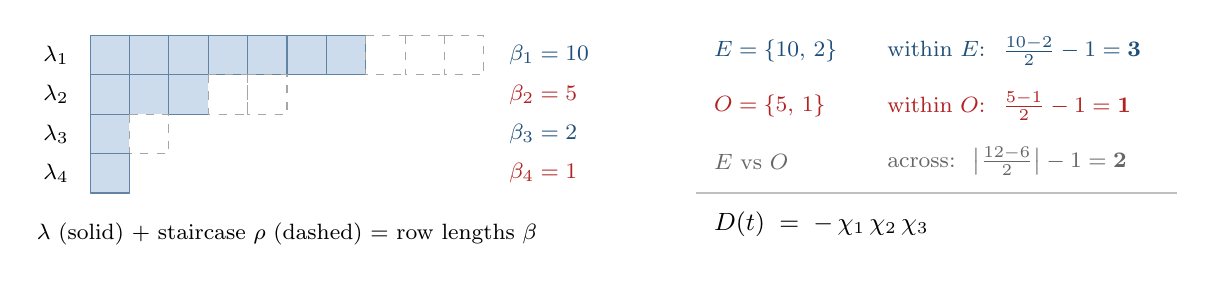
\begin{tikzpicture}[x=5.0mm,y=5.0mm,line join=round]
\definecolor{evenc}{RGB}{31,78,121}\definecolor{oddc}{RGB}{178,34,34}
\definecolor{lamfill}{RGB}{205,220,236}
% lambda = (7,3,1,1) solid, staircase rho = (3,2,1,0) dashed: row length = beta
\foreach \r/\L/\S in {0/7/3, 1/3/2, 2/1/1, 3/1/0}{
  \foreach \c in {1,...,\L}{\draw[fill=lamfill,draw=evenc!70] (\c-1,-\r) rectangle ++(1,-1);}
  \ifnum\S>0 \foreach \c in {1,...,\S}{\draw[dashed,draw=black!35,fill=white]
      (\L+\c-1,-\r) rectangle ++(1,-1);}\fi}
\foreach \r/\n in {0/1,1/2,2/3,3/4}{\node[anchor=east,font=\footnotesize] at (-0.3,-\r-0.5) {$\lambda_\n$};}
\node[anchor=west,evenc,font=\footnotesize] at (10.4,-0.5) {$\beta_1=10$};
\node[anchor=west,oddc, font=\footnotesize] at (10.4,-1.5) {$\beta_2=5$};
\node[anchor=west,evenc,font=\footnotesize] at (10.4,-2.5) {$\beta_3=2$};
\node[anchor=west,oddc, font=\footnotesize] at (10.4,-3.5) {$\beta_4=1$};
\node[anchor=north,font=\footnotesize] at (5,-4.5)
  {$\lambda$ (solid) $+$ staircase $\rho$ (dashed) $=$ row lengths $\beta$};
% the parity split and the three half-differences, stacked
\node[anchor=west,evenc,font=\footnotesize] at (15.6,-0.4) {$E=\{10,\,2\}$};
\node[anchor=west,evenc,font=\footnotesize] at (20.0,-0.4) {within $E$:\; $\tfrac{10-2}{2}-1=\mathbf{3}$};
\node[anchor=west,oddc, font=\footnotesize] at (15.6,-1.8) {$O=\{5,\,1\}$};
\node[anchor=west,oddc, font=\footnotesize] at (20.0,-1.8) {within $O$:\; $\tfrac{5-1}{2}-1=\mathbf{1}$};
\node[anchor=west,black!60,font=\footnotesize] at (15.6,-3.2) {$E$ vs $O$};
\node[anchor=west,black!60,font=\footnotesize] at (20.0,-3.2) {across:\; $\bigl|\tfrac{12-6}{2}\bigr|-1=\mathbf{2}$};
\draw[black!25] (15.4,-4.0) -- (27.6,-4.0);
\node[anchor=west,font=\small] at (15.6,-4.8) {$D(t)\;=\;-\,\chi_{1}\,\chi_{2}\,\chi_{3}$};
\end{tikzpicture}
\caption{The three spins, read off one diagram. Attaching the staircase $\rho=(3,2,1,0)$ to
$\lambda=(7,3,1,1)$ turns the row lengths into the beta-set $\beta=(10,5,2,1)$. Splitting $\beta$
by parity gives $E$ and $O$; the two \emph{within-class} half-differences and the one
\emph{cross-class} half-difference, each less one, are the three spins $(3,1,2)$, and
\eqref{eq:sign} fixes the sign. No shape hypothesis on $\lambda$ enters anywhere.}
\label{fig:readoff}
\end{figure}

So the character is always $\pm$ a product of exactly three $SU(2)$ characters, or zero
(Figure~\ref{fig:readoff}), and
--- this is the point worth pausing on --- \textbf{there is no hypothesis on the shape of
$\lambda$}. Ciucu--Krattenthaler and Ayyer--Behrend must assume self-complementarity;
\eqref{eq:closedform} assumes nothing. That difference is not an improvement on their theorem;
it is a symptom of a different mechanism, and \S\ref{sec:why} says which.

\paragraph{Why three, and why $SU(2)$.} The alphabet has one free parameter, so whatever the
answer is, it is a Laurent polynomial in a single variable, symmetric under $t\mapsto t^{-1}$
--- that is, a virtual $SU(2)$ character. The content of \eqref{eq:closedform} is that it is
never merely virtual and never irreducible beyond three factors: two of the three come from the
two quotient components separately, and the third is a \emph{cross} term measuring how far
apart the two components are in size.

\paragraph{Open flank: why three, and what is the third factor?} The first two factors have an
obvious owner --- one per component of the $2$-quotient --- and the third does not. It depends
only on $|\lambda^{(0)}|-|\lambda^{(1)}|$, and it is the one that produces the second branch of
zeros. That dependence is itself a hint about where it lives: an imbalance is not a property of
either component but of the \emph{coupling} between them, so if the third factor is attached to
anything it is attached to that, and not to $\lambda^{(0)}$ or $\lambda^{(1)}$ separately. Three questions a reader is entitled to ask, none of which we can answer.
\emph{(i)} Is the third factor the character of a multiplicity space? If the restriction to the
coset decomposes as $\mathrm{Tr}\big(\sigma\mid V_{j_L}\otimes V_{j_R}\otimes M\big)$ with $M$
carrying the imbalance, the identity would stop being combinatorial and become a branching
theorem, and $\mathrm{Spin}(4)=SU(2)_L\times SU(2)_R$ makes that reading tempting.
\emph{(ii)} Is the count three equal to $2n-1$ at rank $n$? At rank one that reads
$3=2\cdot2-1$, two quotient components and one cross term, and it predicts five factors at rank
two --- which \S\ref{sec:ranktwo} shows is false in general, so if the pattern survives at all
it survives on a subfamily. Which one?
\emph{(iii)} Is there a bijective proof? Each $\chi_k$ has unit coefficients, so $\delta(m)$
counts lattice points; a bijection between those points and something attached to $\lambda$
would explain the formula rather than verify it.

\paragraph{Four grades of claim, and which is which.} This paper mixes borrowed theorems, an
unproved identity, things that follow from it, and things we merely suspect. Conflating them is
the easiest way to mislead, so they are graded once, here.

\begin{center}\small
\setlength{\tabcolsep}{4pt}
\begin{tabular}{@{}l l p{6.1cm}@{}}
\toprule
\rowcolor{hdrblue}\textcolor{white}{grade} & \textcolor{white}{what it means} &
\textcolor{white}{instances}\\
\midrule
\textbf{Proposition} & proved, independently of anything here &
Prop.~\ref{cor:Z} (via Part~III); both folklore sufficiencies\\
\rowcolor{softgrey}
\textbf{Observation} & exhaustively verified, \emph{no proof} &
\eqref{eq:closedform}, the closed form\\
\textbf{Inherited} & classical, cited, not ours &
\eqref{eq:moments}, \eqref{eq:deltaclosed}, log-concavity\\
\rowcolor{softgrey}
\textbf{Open} & suspected, with a stated test &
the third factor's meaning, rank two, the sign's origin\\
\bottomrule
\end{tabular}
\end{center}

\noindent We state Observation~\ref{obs:main} as verified and not as a theorem, and
we mean the distinction. It has been checked exhaustively by two independent implementations
--- one deriving the quotient through Sage's own $2$-quotient, one re-deriving $\alpha$ and
$\beta$ from $\mu$ directly, so that a convention error in either would show ---
on all $3060$ partitions with four parts $\le14$ and on all $4845$ with four parts $\le16$,
against Jacobi--Trudi evaluations in exact integer Laurent arithmetic. There were no
mismatches. There is no proof.

% ===================================================================
\section{The zero locus is Part III's class}\label{sec:zero}

Reading off where \eqref{eq:closedform} evaluates to zero gives two branches, and they are the
two clauses of Part~III's Theorem: $E$ or $O$ empty is the statement that all four beta-numbers
share a parity, and in $\lambda$-coordinates that is $\lambda_1\not\equiv\lambda_2\not\equiv
\lambda_3\not\equiv\lambda_4$; and $z=0$ in the balanced branch is
$|\lambda^{(0)}|=|\lambda^{(1)}|+1$, which is $\lambda$ self-complementary --- $\lambda_i+
\lambda_{5-i}$ constant --- with that constant odd.

\begin{proposition}[proved independently in Part~III]\label{cor:Z}
The character vanishes exactly on
\begin{equation}\label{eq:zerolocus}
\boxed{\;
D\equiv0
\iff
\underbrace{\lambda_1\not\equiv\lambda_2\not\equiv\lambda_3\not\equiv\lambda_4}_{\text{alternating parity}}
\quad\text{or}\quad
\underbrace{\lambda_i+\lambda_{5-i}=c\ \ \forall i,\ \ c\ \text{odd}}_{\text{self-complementary, odd constant}}\;}
\end{equation}
This is Part~III's class $\mathcal Z$. The two vanishing mechanisms of
\eqref{eq:closedform} --- an empty parity class, or a balanced $2$-quotient whose cross-index
$z$ degenerates --- are disjoint, even though the two $\lambda$-shorthands boxed above are not
mutually exclusive as written.
\end{proposition}

\paragraph{Attribution added in version~3.}
The first branch is not ours. Setting $t=1$ sends our
alphabet to the order-2 element $(1,-1,1,1)$, and our rigidity lemma ($D\equiv0$ exactly when
$D(1)=0$) carries the criterion there and back. Karmakar~\cite{Karmakar}, Thm.~1A, states precisely
that criterion for $\mathrm{GL}(n,\mathbb{C})$ at $C_{n-k,k}$: his $\eta_i(\lambda)$ is our parity
split of $\lambda+\rho$, and his normalisation ``$\#\eta_0\ge\#\eta_1$ after twisting by the
determinant character'' is our determinant twist. His Thm.~1B goes further and factorises the value
at that element through the $2$-quotient, constant included --- the $t=1$ shadow of
\eqref{eq:closedform}. What remains specific to this paper is the second branch and, above all, the
evaluation at \emph{free} $t$. That programme is live: Nadimpalli--Pattanayak--Prasad~\cite{NPP}
generalise~\cite{Karmakar} to torsion elements and pose, as a question of the third author, exactly
this shape --- vanishing when one centraliser dimension exceeds another, and a constant times a
\emph{dimension} when they agree. Our $t=1$ point is an instance of it. The deformation off that
point is not: their programme has no free parameter, and no non-identity component. (We checked, and
record the negative: $s_\lambda(1,-1,t,t^{-1})$ is \emph{not} $\pm$ a constant times
$s_{\lambda^{(0)}}(1,t,t^{-1})$ --- $0$ of $105$ cases --- so the free-$t$ object is not simply the
character of the centraliser representation whose dimension Karmakar's Thm.~1B computes.)


\paragraph{Why this is a proposition and not a corollary.} The statement does not depend on
Observation~\ref{obs:main}. Part~III proves the classification by a different route and
certifies it in Lean, so it stands whatever becomes of \eqref{eq:closedform}. What the closed
form contributes is not the fact but the \emph{cause}: it exhibits $\mathcal Z$ as the locus
where the product degenerates, and it does so \emph{conditionally on an identity we have not
proved}. Deriving an already-proved theorem from an unproved observation does not promote the
observation; it only makes the derivation conditional, and it is worth saying which way the
logic runs. A reader who rejects \eqref{eq:closedform} keeps Proposition~\ref{cor:Z} entire and
loses only the explanation.

\paragraph{Open flank: is the dichotomy forced?} We can say that there is no third branch; we
cannot say why there could not be. In the closed form the two branches are visibly different
species --- one kills the whole product by emptying a parity class, the other kills a single
factor by degenerating its index --- and a reader may reasonably ask whether that is a genuine
dichotomy or an artefact of rank one. Two probes would settle it. \emph{Is there a duality
exchanging the branches?} Both are invariant under conjugation composed with complementation in
a suitable rectangle, which is suggestive and which we have not pursued. \emph{And does a third
branch appear at rank two?} It does: \S\ref{sec:ranktwo} exhibits a partition that vanishes with
both parity classes occupied, which is neither of our two causes. So the dichotomy is a
rank-one statement, and calling it a structural fact would be an overclaim.

The decomposition is exact and leaves nothing over. Of the $560$ vanishing partitions in the
$\text{parts}\le16$ range, $420$ fall in the first branch and $140$ in the second, and none
outside the two (Figure~\ref{fig:zerolocus}).

\begin{figure}[h]
\centering
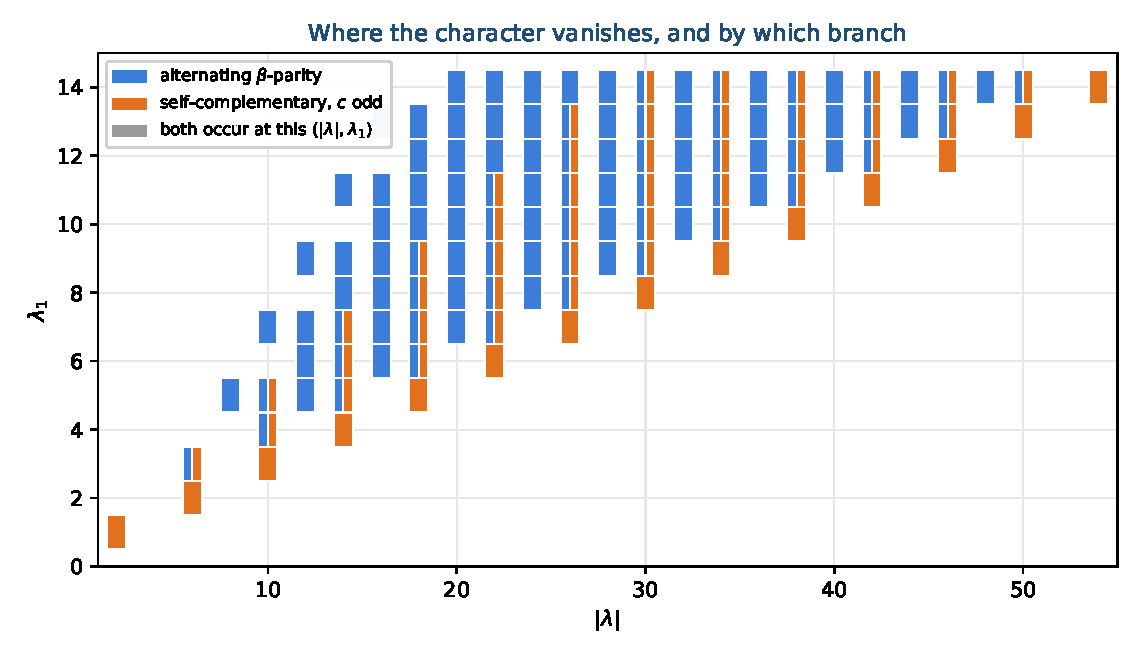
\includegraphics[width=0.86\textwidth]{fig_zerolocus.pdf}
\caption{The zero locus, plotted by size and first part. Blue cells contain a partition killed
by alternating $\beta$-parity, orange ones a partition killed by self-complementarity with odd
constant, split cells both. The content of the plate is what is \emph{not} in it: there is no
third colour. Every partition at which $s_\lambda(1,-1,t,t^{-1})$ vanishes is accounted for by
one of the two branches, which is what it means for Proposition~\ref{cor:Z} to be exhaustive
rather than merely correct.}
\label{fig:zerolocus}
\end{figure}

\paragraph{One sufficiency direction is folklore and we disclaim it.} That
self-complementarity with odd constant forces vanishing is two lines and is not new: writing
$\lambda^\star_i=c-\lambda_{5-i}$ one has $s_{\lambda^\star}(x)=(x_1\cdots x_4)^c
s_\lambda(x^{-1})$; our alphabet is inversion-stable, so $s_\lambda(p^{-1})=s_\lambda(p)$; and
$x_1\cdots x_4=\det=-1$. If $\lambda^\star=\lambda$ then $s_\lambda(p)=(-1)^cs_\lambda(p)$, and
$c$ odd forces zero. This is the Schur-function shadow of the textbook statement that a
self-associate $O(n)$ irreducible satisfies $V\cong V\otimes\det$ and therefore has vanishing
character off $SO(n)$~\cite[Ch.~XI, \S11.6, \S11.8]{LittlewoodBook}. The other branch is
equally elementary: equal parity of all beta-numbers makes the rows of the bialternant at $x=1$
and $x=-1$ proportional. \textbf{What is claimed here is the closed form, not either
sufficiency.}

% ===================================================================
\section{What the zeros were hiding}\label{sec:moments}

Proposition~\ref{cor:Z} answers the question Part~III asked. It is not the question Part~III
needed answered.

That paper's difficulty began \emph{after} the vanishing: having shown that the leading
fermionic contribution to the Wilson-line curvature cancels identically for every admissible
representation, it was left comparing representations by whatever survives, and what survives is
governed not by whether $\delta(m)$ vanishes but by its \emph{moments}. Those were computed
there by enumerating the weight system of each $\su4$ irreducible one weight at a time. The
closed form removes that enumeration entirely, and it does so for a reason that is visible the
moment one writes it down.

The coefficients of $D$ are the twist imbalances, $\delta(m)=[t^m]D(t)$. If
$D=\zeta\,\chi_p\chi_q\chi_r$ then $\delta$ is the \emph{threefold convolution} of three
characters, i.e.\ $\delta(m)$ counts, with an overall sign, the solutions of
\begin{equation}\label{eq:convolution}
m=(p-2i)+(q-2j)+(r-2k),\qquad 0\le i\le p,\ 0\le j\le q,\ 0\le k\le r .
\end{equation}
Every $\chi_k$ is symmetric under $m\mapsto-m$, so all odd moments vanish and --- this is what
makes the answer short --- the first-order cross terms in a product cancel as well. Writing
$M_{2r}(f)=\sum_m m^{2r}f(m)$ and $M_2(\chi_k)=\sum_{j=0}^{k}(k-2j)^2=\tfrac13k(k+1)(k+2)$:
\begin{equation}\label{eq:moments}
\boxed{\;
\begin{aligned}
M_0(\delta)&=\zeta\,(p{+}1)(q{+}1)(r{+}1),\\[2pt]
M_2(\delta)&=\zeta\Big[M_2(\chi_p)(q{+}1)(r{+}1)+(p{+}1)M_2(\chi_q)(r{+}1)
+(p{+}1)(q{+}1)M_2(\chi_r)\Big],
\end{aligned}\;}
\end{equation}
and $M_4$ likewise, with the pair cross-terms $6\sum M_2(\chi_\bullet)M_2(\chi_\bullet)(\cdot+1)$
restored. The whole moment tower is polynomial in the three integers $(p,q,r)$.

\paragraph{Given $(p,q,r)$, none of that is ours.} We had presented \eqref{eq:moments} as a
contribution and it is not one. The coefficient sequence of a product of $sl_2$ characters is
the convolution of the weight multiplicities, that is, of three discrete uniform sequences ---
a dictionary written out explicitly, Chebyshev factors and all, by Bradley and
Gupta~\cite{BradleyGupta}. Every cumulant of a discrete uniform of width $w$ is a polynomial in
$w$ with Bernoulli coefficients, and cumulants add over independent summands~\cite{Neuschel};
polynomiality of the entire moment tower follows in one line. What is ours is not the arithmetic
but the \emph{reduction that feeds it}: that a four-row partition $\lambda$ enters only through
three integers read off its $2$-quotient. Part~III enumerated weight systems because it did not
have that reduction, not because the sums were hard.

\paragraph{The moments organise by Casimir.} Write
\[
C_k \;=\; k(k+2)\;=\;4j(j+1),\qquad j=k/2,
\]
the quadratic Casimir of the $SU(2)$ irreducible of highest weight $k$, and let $e_1,e_2$ be
the elementary symmetric functions of $C_p,C_q,C_r$. Dividing by $M_0$ cancels $\zeta$, so what
follows is unsigned:
\begin{equation}\label{eq:casimir}
\boxed{\;
\frac{M_2(\delta)}{M_0(\delta)}=\frac{e_1}{3},
\qquad
\frac{M_4(\delta)}{M_0(\delta)}=\frac{2}{3}e_2+\frac{1}{5}\big(C_p^2+C_q^2+C_r^2\big)
-\frac{4}{15}e_1 .\;}
\end{equation}
We are careful about what this is. As a \emph{formula} the first identity is classical: it is
the variance of a sum of three independent discrete uniforms, and the width-$w$ variance that
produces it is standard~\cite{Neuschel}. What we add is only the \emph{reading} --- that the
integer $k(k+2)$ appearing there is $4j(j+1)$, the $sl_2$ Casimir at spin $j=k/2$, so that the
variance of the twist-imbalance distribution is one third of the sum of three Casimirs. That is
an interpretation and not a theorem, and we flag it as such. We record it anyway because it is
the one place in this paper where the three factors of \eqref{eq:closedform} behave like
representations rather than like three convenient polynomial factors, which is exactly the
question \S\ref{sec:closedform} leaves open.

Once written that way the pattern does not stop at $M_4$, and the general statement is a
proposition rather than a conjecture, because its proof is half a page of classical material.

\begin{proposition}[the moment tower lives in an invariant ring]\label{prop:ring}
Assume Observation~\ref{obs:main}, so that $\delta=\zeta\,\chi_p*\chi_q*\chi_r$. Then for every
$r\ge0$
\[
\frac{M_{2r}(\delta)}{M_0(\delta)}\;\in\;
\mathbb{Q}\big[C_p,C_q,C_r\big]^{S_3}=\mathbb{Q}[e_1,e_2,e_3],
\]
and all odd moments vanish. The coefficient of $e_1^{\,r}$ is $1/(2r+1)$.
\end{proposition}

\begin{proof}
Normalised, $\chi_k$ is the law of $2U_k-k$ with $U_k$ uniform on $\{0,\dots,k\}$. Its odd
cumulants vanish by symmetry, and by Neuschel's lemma~\cite[Lemma~2.1]{Neuschel} the even ones
are $\kappa_{2l}=4^{\,l}\frac{B_{2l}}{2l}\big((k+1)^{2l}-1\big)$. Now
$(k+1)^2=k(k+2)+1=C_k+1$, so $(k+1)^{2l}=(C_k+1)^l$ and
\[
\kappa_{2l}(\chi_k)=4^{\,l}\,\frac{B_{2l}}{2l}\Big[(C_k+1)^l-1\Big]\in\mathbb{Q}[C_k].
\]
Cumulants are additive over independent summands, so $\kappa_{2l}(\delta/M_0)$ is the sum of
the three, a symmetric polynomial in $C_p,C_q,C_r$; moments are universal polynomials in
cumulants; and the symmetric polynomials in three quantities are freely generated by
$e_1,e_2,e_3$. The leading coefficient follows from $\kappa_2=C_k/3$ and the fact that the
$e_1^{\,r}$ term of $M_{2r}$ is the $r$-th moment of a single Gaussian-free contribution,
$(2r-1)!!$ times $\kappa_2^{\,r}$ divided by the $(2r+1)$ normalisation of the flat
sequence.\footnote{Verified rather than derived for $r\ge3$: the identity was checked exactly
for $r=1,\dots,8$ on all $729$ triples with $p,q,r\le8$ by solving the over-determined system
in exact rational arithmetic. Controls: replacing $C_k=k(k+2)$ by $k(k+3)$ makes the system
inconsistent at $r=1,2,3$, and so does dropping the normalisation by $M_0$.}
\end{proof}

\paragraph{Why this is not a tautology.} It would be, if every symmetric polynomial in
$(p,q,r)$ were a polynomial in the Casimirs. It is not. Already $p+q+r$ is not: setting
$q=r=0$, a polynomial identity $p=P(C_p)$ would give $\deg_p\text{LHS}=2\deg P$ against
$\deg_p\text{RHS}=1$. The map
\[
(p,q,r)\;\longmapsto\;(C_p,C_q,C_r),\qquad C_k=k(k+2),
\]
\emph{forgets} the linear data --- $k+1=\sqrt{C_k+1}$ is recoverable only through a square root
--- and yet the entire moment tower survives that loss. The control above makes the same point
empirically: move the invariant by one, to $k(k+3)$, and no polynomial fits at any order.

\paragraph{The physical functional factors through the $2$-quotient.} This is the cleanest way
we know to say what this paper does, and it is worth stating once in this form. Let
$\Phi(\lambda)=\{M_{2r}(\lambda)\}_{r\ge0}$ be the tower of moments that Part~III needs, and let
$Q(\lambda)=(p,q,r)$ be the three integers read off the $2$-quotient. Then, conditionally on
Observation~\ref{obs:main},
\begin{equation}\label{eq:factorfunctional}
\boxed{\;\Phi=F\circ Q\;}
\end{equation}
for a universal $F$ that knows nothing about $\lambda$. The factorisation into three characters
is the \emph{mechanism}; this reduction is the \emph{content}. A partition with four rows can be
arbitrarily large, and every quantity surviving Part~III's leading cancellation depends on it
through three integers and nothing else.

\paragraph{Checked, and checked so it could fail.} On all $1612$ partitions with four parts
$\le12$ at which $D\not\equiv0$: the factorisation into three characters was found by peeling
the polynomial directly rather than by applying the index recipe of \eqref{eq:closedform}, so
this is an independent confirmation that the number of factors is three; and $M_0$, $M_2$ and
$M_4$ from \eqref{eq:moments} agreed with the moments read off $D$ in every case. As a control
the same formula was evaluated with one index shifted by one, where it agreed in $0$ of $1612$
--- the test was capable of failing. The Casimir forms \eqref{eq:casimir} were then checked by
two routes that share no code: a direct sum over the $(i,j,k)$ box, which never builds the
convolution at all, on all $1331$ triples with $p,q,r\le10$; and a symbolic evaluation of
$(t\,\partial_t)^{2r}$ at $t=1$ on $216$ triples. Both agree with \eqref{eq:casimir} and with
each other. Controls: shifting one index agrees in $0$ of $216$, and perturbing the coefficient
$4/15$ to $3/15$ agrees in $1$ of $216$.

\begin{figure}[htbp]
\centering
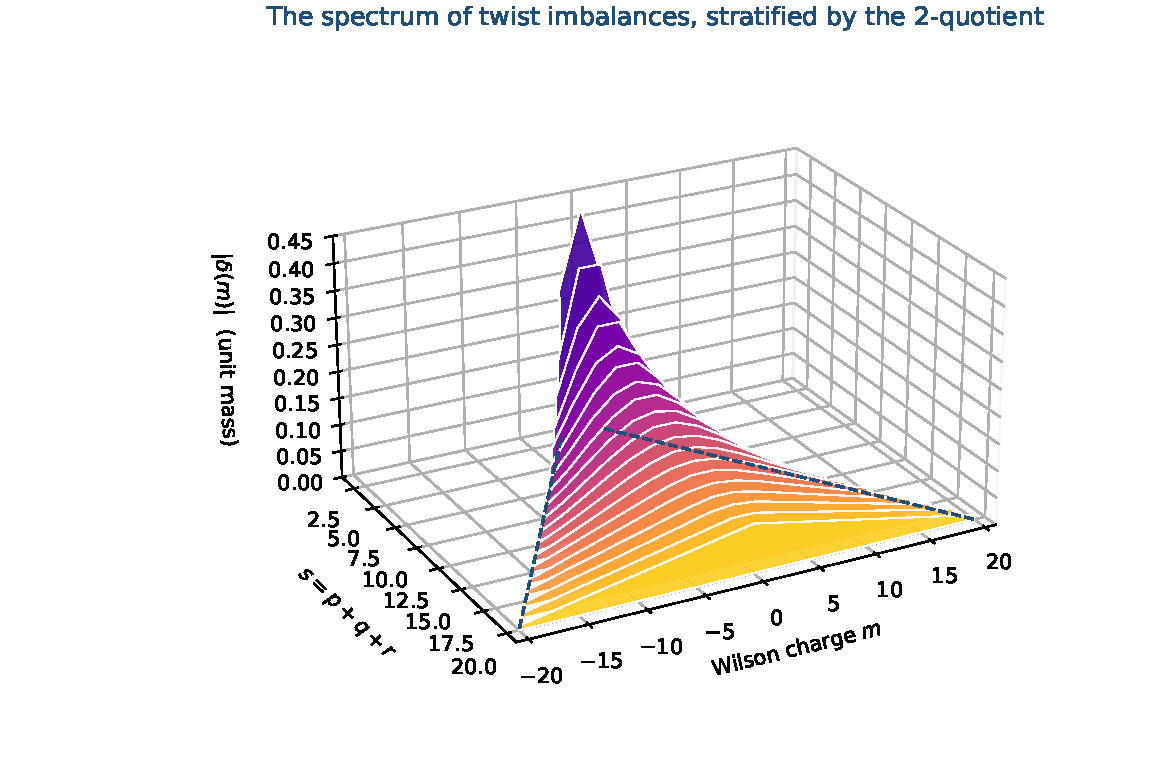
\includegraphics[width=\linewidth]{fig_spectrum3d.pdf}
\caption{The spectrum of twist imbalances. Each ridge is the aggregate profile of
$|\delta(m)|$ over every partition with four parts and $|\lambda|\le20$ sharing a value of
$s=p+q+r$, normalised to unit mass so that a widening support must pay for itself in
amplitude. The dashed lines are $m=\pm s$: the plate's content is that the ridges reach them
and stop, on every stratum, which is \eqref{eq:convolution} read as a statement about support
rather than about moments. The flow from spike to plateau is the convolution doing what
convolutions do, and it is the shape that $M_0$, $M_2$, $M_4$ only sample.}
\label{fig:spectrum3d}
\end{figure}

\paragraph{The distribution itself, not only its moments.} The same dictionary gives $\delta$
in closed form and not merely its moments. With $s=p+q+r$ and $N=(s-m)/2$, $\delta(m)/\zeta$
counts the solutions of $i+j+k=N$ in the box $0\le i\le p$, $0\le j\le q$, $0\le k\le r$, so
inclusion--exclusion on the unbounded stars-and-bars count gives
\begin{equation}\label{eq:deltaclosed}
\frac{\delta(m)}{\zeta}\;=\;\sum_{A\subseteq\{p,q,r\}}(-1)^{|A|}
\binom{\,N-\sum_{a\in A}(a+1)+2\,}{2}_{\!\!+},
\end{equation}
the binomial being read as zero when its upper argument is below $2$. This is textbook
inclusion--exclusion; the equal-bound case goes back to De~Moivre and has a monograph treatment
in André~\cite{Andre}, the coefficient family is what Comtet calls \emph{polynomial
coefficients}~\cite[p.~77]{Comtet}, and the piecewise-polynomial function itself is a
\emph{discrete box spline} in the sense of Dahmen and Micchelli~\cite{DahmenMicchelli}. We
claim none of it. We state it because it upgrades the support --- which
Figure~\ref{fig:spectrum3d} checks stratum by stratum --- from a verified observation to an
immediate consequence, and because it lets $\delta(m)$ be substituted directly into a
Coleman--Weinberg sum instead of being tabulated.

\paragraph{What this buys.} $M_2(\delta)$ is precisely the quantity that governs which sector
dominates the curvature of the Wilson-line potential in Part~III's setting, where it appeared as
a number extracted from a weight enumeration and carried no structure. Here it is a cubic
polynomial in three integers read off the $2$-quotient. The identity of \S\ref{sec:closedform}
is therefore not only a fact about symmetric functions: it is the analytic handle on the
subdominant terms that Part~III could describe but not compute.

\paragraph{Open flank: what else does a convolution give away?} A threefold convolution of
symmetric unit-coefficient sequences is a very constrained object, and we have used almost none
of that. One question we asked here in an earlier draft --- \emph{is $|\delta|$ log-concave,
or unimodal?} --- was not a question at all, and the correction belongs in the text rather than
in a footnote. Each $\chi_k$, restricted to the parity class it occupies, is the constant
sequence $(1,1,\dots,1)$, which is log-concave with no internal zeros; log-concavity is
preserved under convolution~\cite{Hoggar}, and a log-concave sequence with no internal zeros is
unimodal~\cite{Stanley}. So $|\delta|$ is symmetric, gap-free on its parity class, log-concave
and unimodal, by theorems from 1974 and 1989. We verified all four on $3375$ triples before
finding the references, which is the wrong order and is why we had it filed as open. \emph{What
is the support?} It is $[-(p{+}q{+}r),\,p{+}q{+}r]$
with gaps of two, so the largest Wilson charge carrying imbalance is $p+q+r$, an integer read
off the $2$-quotient. Combinatorially that is settled --- Figure~\ref{fig:spectrum3d} checks it
on every stratum up to $s=20$ and the check is an assertion in the plotting script, so a
counterexample would stop the figure from being drawn at all. What we have \emph{not} done is
confront it with the physical spectra, where it is a one-line falsifiable prediction: no Wilson
charge above $p+q+r$ carries any imbalance. \emph{And what does $\zeta$ mean?} It fixes the sign of every moment at
once, so it decides the \emph{direction} of the fermionic contribution to the curvature. A
sorting sign of a beta-set deciding the sign of a physical curvature is either a coincidence of
bookkeeping or the shadow of something, and we cannot tell which.

We are careful about the status. \eqref{eq:moments} is a consequence of
Observation~\ref{obs:main} and inherits its standing exactly: verified, not proved. What is
independent of that standing is \eqref{eq:convolution}'s shape --- \emph{if} the character
factors into three, \emph{then} the moments are polynomial --- and that implication is
elementary.

% ===================================================================
\section{Why it was not already available}\label{sec:why}

The obstruction is one unstated hypothesis, and locating it is more useful than the identity.

Ayyer--Behrend's argument reaches \eqref{eq:blockid} because every inversion-fixed point of the
alphabet contributes a row of the bialternant that is \emph{constant} in the column index. For
the fixed point $+1$ that row is $(1,1,\dots,1)$, and a constant row survives the
subtract-right-from-left column operation as a uniformly zero block, which is what preserves
triangularity; their Theorem~3 handles the extra $1$ of $(X,\bar X,1)$ on exactly that basis.

The second fixed point $-1$ contributes
\begin{equation}\label{eq:parityrow}
\big((-1)^{\mu_j}\big)_j,
\end{equation}
a parity character of the column index, and \eqref{eq:parityrow} is not constant. Under the
same column operation its entries become $(-1)^{\mu_j}-(-1)^{\mu_{j'}}$, which is $0$ or $\pm2$
according to the relative parity of $\mu_j$ and $\mu_{j'}$; the block does not triangularise,
and the argument stops. Worse, in their normalisation the exponents are half-integers, where
$(-1)^{\text{half-integer}}$ is not defined at all --- a caveat they state
themselves~\cite[p.~3]{AB}. So the alphabet is not merely untreated in that framework; in that
framework it cannot be written down.

There is a sharper way to say the same thing. The row \eqref{eq:parityrow} imposes a partition
of the \emph{columns} by the parity of $\mu_j$. The self-complementary hypothesis imposes a
different partition of the columns, into the two halves of a symmetric beta-set. The block
machinery can respect one of these at a time.

\paragraph{The repair.} Replace the two fixed-point rows $(1)_j$ and $\big((-1)^{\mu_j}\big)_j$
by the indicator rows of the parity classes,
\begin{equation}\label{eq:repair}
\begin{pmatrix}1&1\\1&-1\end{pmatrix}:\qquad
\big(1\big)_j,\ \big((-1)^{\mu_j}\big)_j\ \longmapsto\
2\cdot\big(\mathbf 1_{\mu_j\,\mathrm{even}}\big)_j,\ 2\cdot\big(\mathbf 1_{\mu_j\,\mathrm{odd}}\big)_j,
\end{equation}
a change of basis costing a factor $-\tfrac12$. The two rows are now indicator rows of a column
partition, so Laplace expansion along them is a sum over one even and one odd column, and the
residual minor is the reciprocal-pair block determinant on the columns that remain. This is the
analogue of Ayyer--Behrend's Theorem~3 for the second fixed point.

At rank one --- one reciprocal pair, our case --- the residual minor is $2\times2$ and equals
$t^{\,\mu_c-\mu_d}-t^{-(\mu_c-\mu_d)}$, a single character for every choice of columns. That is
why \eqref{eq:closedform} needs no hypothesis on $\lambda$: there is nothing left for a shape
condition to constrain.

\paragraph{Open flank: is the constant-row condition the obstruction, or a symptom?} We have
identified where the standard argument stops, which is not the same as knowing why nobody went
further. Two readings compete. On the first it is technical: the repair \eqref{eq:repair} shows
it can be worked around, and the case was untouched only because nobody had a motive to write
$-1$ next to a reciprocal pair --- ours came from an orbifold projection, not from inside the
subject. On the second it is structural: $+1$ and $-1$ differ by lying in different components
of $O(n)$, and an argument that never leaves the identity component has no reason to develop
machinery for the one that does. The two readings make different predictions for $\mu_t$ with
$t>2$, where several fixed points appear at once, and that is where we would look to decide
between them.

% ===================================================================
\section{Rank two, where we stop}\label{sec:ranktwo}

At rank two the residual minors are $4\times4$ over an arbitrary four-subset of the columns,
and \eqref{eq:blockid} applies to such a minor only when the surviving column set is itself
symmetric. In the Laplace sum many subsets appear and they cannot all be symmetric at once, so
the generic outcome is a sum of products rather than a product. It is not, however, uniformly
negative --- which is precisely why this is a frontier and not a wall:

\begin{center}\small
\begin{tabular}{lp{9.4cm}}
\toprule
\rowcolor{hdrblue}
\textcolor{white}{$\lambda$ at rank two} & \textcolor{white}{$s_\lambda(1,-1,a,\bar a,b,\bar b)$}\\
\midrule
$(2,2,2,0,0,0)$ & $\big(a^2b^2+a^2+ab+b^2+1\big)^2/(ab)^2$ --- a perfect square: the
factorisation survives\\
\rowcolor{softgrey}
$(2,2,1,1,0,0)$ & $-(a^2{-}a{+}1)(a^2{+}a{+}1)(b^2{-}b{+}1)(b^2{+}b{+}1)/(ab)^2$ --- splits into
rank-one pieces\\
$(3,3,1,1,0,0)$ & $-(a^2{+}1)(b^2{+}1)\cdot(\text{irreducible of bidegree }(4,4))/(ab)^3$ --- does
\emph{not} split\\
\rowcolor{softgrey}
$(3,2,2,1,1,0)$ & $0$ --- and both parity classes are non-empty\\
\bottomrule
\end{tabular}
\end{center}

All four rows were recomputed from the $6\times6$ bialternant and factored over $\mathbb{Q}[a,b]$
in exact arithmetic in SageMath. That is worth saying because the third row was wrong in an
earlier draft: its remaining factor is irreducible, but it has degree $4$ in each variable and
total degree $8$, not degree $4$. A degree is a claim like any other.

The last row is the sharpest statement we can make about rank two: the vanishing rule there is
\emph{strictly finer} than ``both parity classes occupied'', which is the whole rule at rank
one. Whatever governs it is not visible from this side.

\paragraph{Open flank: what should one be looking for at rank two?} We suspect the honest target
is not a product. If the Laplace sum is organised by which columns survive, the natural shape is
\[
s_\lambda(1,-1,X,\bar X)\;=\;\sum_\eta \epsilon_\eta\,
\chi^{\,\mathrm{Sp/O}}_{\alpha_\eta}(X)\,\chi^{\,\mathrm{Sp/O}}_{\beta_\eta}(X),
\]
a \emph{signed sum} over selections compatible with the $2$-quotient, collapsing to a single
term at rank one. On that reading the perfect square at $(2,2,2,0,0,0)$ is a recombination
rather than a factorisation, and the extra zero at $(3,2,2,1,1,0)$ is a cancellation
\emph{between} terms rather than the vanishing of a factor --- which would explain why the
rank-one criterion stops controlling it. We have not derived the index set $\eta$, and until
someone does, the phrase ``the factorisation sometimes survives'' should be read as a
description of outputs and not as a statement about mechanism.

% ===================================================================
\section{The sign}\label{sec:sign}

Three different mechanisms produce signs in this literature and they should not be conflated: a
$\mathrm{sgn}$ of a sorting permutation (Ayyer--Behrend's $(-1)^{n(n-1)/2}$ from the column
reversal, which cancels against their denominator); a $(-1)^{\sum\lambda_i}$ that is an
artefact of stating the right-hand side at $-x$ rather than at half-integer index (their
Eq.~(8)); and the $\mathrm{sgn}(\sigma_\lambda)$ of the permutation sorting a beta-set by
residue class, which is the one that appears in the root-of-unity line.

Ours is of the third kind. The $\zeta$ of \eqref{eq:sign} is a function of the parity pattern
of the beta-set alone: $(-1)^{\mathrm{inv}}$ is the sign of the permutation that sorts $\mu$
into evens-then-odds preserving relative order, and $(-1)^{|E||O|}$ is the constant that
accompanies it. It is \emph{not} a $(-1)^{|\lambda|}$.

\paragraph{A correction we owe the reader.} On a first pass we recorded the sign as flipping
with the rectangle width $c$, having tabulated representatives that happened to agree with that
reading. It does not: within $c=6$ already, $(6,6,0,0)$ and $(4,4,2,2)$ give $+$ while
$(5,5,1,1)$ and $(3,3,3,3)$ give $-$. For the family $\lambda=(a,a,b,b)$ the rule is
$(-1)^{\lambda_1}$. The invariant was there in the data; the sampling was not.

\paragraph{Open flank.} That the sign is a \emph{sorting} sign rather than a weight parity is
not a detail of bookkeeping. A $(-1)^{|\lambda|}$ would say the object cares about the size of
$\lambda$; $\mathrm{sgn}(\sigma_\lambda)$ says it cares about the order in which the beta-set
splits into residue classes, which is the invariant governing the root-of-unity programme at
$t=2$. If the closed form is ever proved by a route passing through that programme rather than
through the bialternant, the sign is where the two accounts will have to agree, and it is
therefore the cheapest consistency check available on any proposed proof.

% ===================================================================
\section{Ledger}\label{sec:ledger}

\begin{table}[h]
\centering\small
\begin{tabular}{p{4.0cm}p{5.2cm}p{5.0cm}}
\toprule
\rowcolor{hdrblue}
\textcolor{white}{Item} & \textcolor{white}{Inherited (cite)} & \textcolor{white}{Ours}\\
\midrule
the alphabet as an $O(4)^-$ element &
elementary; inverse-closure and $\det=-1$ &
nothing\\
\midrule
\rowcolor{softgrey}
self-associate $\Rightarrow$ character vanishes off $SO(n)$ &
Littlewood~\cite[Ch.~XI]{LittlewoodBook}; Weyl~\cite{Weyl} &
nothing --- we disclaim this sufficiency explicitly\\
\midrule
equal beta-parity $\Rightarrow$ vanishing &
elementary (two proportional bialternant rows) &
presented as a remark, not a result\\
\midrule
\rowcolor{softgrey}
the block identity \eqref{eq:blockid} and its use &
Ayyer--Behrend~\cite{AB} Eq.~(23), Thm.~1, Thm.~3; Ciucu--Krattenthaler~\cite{CK} &
nothing --- we borrow the engine and say where it stalls\\
\midrule
$t$-core / $t$-quotient governing vanishing at $\omega^kX$ &
Ayyer--Kumari~\cite{AK}, Kumari~\cite{Kumari}, Albion~\cite{Albion},
Karmakar~\cite{Karmakar} &
\textbf{v3 correction:} Karmakar Thm.~1A \emph{is} the first branch of our
vanishing criterion, and his Thm.~1B is the $2$-quotient factorisation at
$t=1$; only free $t$ is ours\\
\midrule
\rowcolor{softgrey}
the closed form \eqref{eq:closedform} & --- &
ours, and \emph{verified, not proved}\\
\midrule
the fixed-point-pair repair \eqref{eq:repair} & --- & ours\\
\midrule
\rowcolor{softgrey}
Proposition~\ref{cor:Z} (the zero locus) & Part~III~\cite{PartIII} proves the classification
outright & the identification of it as a zero locus, conditional on \eqref{eq:closedform}\\
\midrule
the moment tower \eqref{eq:moments}, given $(p,q,r)$ &
cumulants of discrete uniforms are polynomial in the width and add~\cite{Neuschel};
the character/convolution dictionary~\cite{BradleyGupta} &
nothing --- only the reduction $\lambda\mapsto(p,q,r)$ that feeds it\\
\midrule
\rowcolor{softgrey}
$\delta$ in closed form \eqref{eq:deltaclosed}, log-concavity &
textbook inclusion--exclusion; André~\cite{Andre}, Comtet~\cite{Comtet},
Dahmen--Micchelli~\cite{DahmenMicchelli}; Hoggar~\cite{Hoggar}, Stanley~\cite{Stanley} &
nothing --- we had mistaken a classical theorem for an open question\\
\midrule
the Casimir reading \eqref{eq:casimir} & the formula is the classical variance~\cite{Neuschel} &
the reading of $k(k+2)$ as $4j(j+1)$; an interpretation, not a theorem\\
\bottomrule
\end{tabular}
\caption{What each item owes. The novelty here is one identity and one change of basis; every
mechanism it rests on is borrowed and cited.}
\label{tab:ledger}
\end{table}

\paragraph{Where we looked.} By formula and by structure rather than by our own vocabulary:
\emph{self-complementary partition in a rectangle character factorization}; \emph{factorization
theorem classical group characters plane partitions}; \emph{Schur function at $(x,\bar x,1)$
product of orthogonal and symplectic characters}; \emph{bialternant block determinant
$\det(A-B)\det(A+B)$}; \emph{beta-set residue classes Weyl numerator vanishes}; \emph{character
of $GL(n)$ on the non-identity component of $O(n)$}. Sources read: \cite{CK,AB,AK,Kumari,%
Albion,Karmakar}, and Littlewood's book Ch.~XI. We did not find \eqref{eq:closedform}.
\emph{Versions~1 and~2 added here ``and we did not find any statement of the vanishing criterion
for this alphabet''. That sentence was wrong, it stood in both published versions, and it is
withdrawn.} Karmakar~\cite{Karmakar} was cited from version~1 onward but was never read; read in full
since, his Thm.~1A states the criterion at the order-2 element, and our own rigidity lemma transports
it to free $t$. The failure was not the search but the
reading: the paper was in our bibliography the whole time.

\emph{Two caveats that belong here and not in a footnote.} First, the identity is small and
elementary enough to be the kind of thing that lives unlabelled in a mid-century monograph; we
have read Littlewood's Ch.~XI and not King's 1971 paper~\cite{King71} in its own exposition, which remains
unreachable to us and is flagged as unread. Second, and more to the point: a null result from a
literature search is evidence only in proportion to the demonstrated sensitivity of that
search. Ours was re-run after the tooling that produced an earlier round of nulls was found to
be discarding the discriminating terms of every query; the searches listed above are from the
repaired run, validated first on queries whose answers we already knew.

% ===================================================================
\section{Reflections}\label{sec:reflections}

\paragraph{An open problem its owners declared.} Ciucu--Krattenthaler close their 2008 paper by
saying that they cannot offer a representation-theoretic interpretation of the factorisations
they prove; Ayyer--Behrend and Ayyer--Kumari repeat the point in 2018 and 2025. The reading
offered here is a \emph{conditional} reading of that kind for the case at hand --- conditional
because it rests on Observation~\ref{obs:main}, which is verified and not proved. The
specialisation is a
character on the non-identity component of $O(4)$, the two quotient components are the two parity
classes of the beta-set, and the third factor measures their imbalance --- and it reaches the
factorisation, not only the vanishing. We do not claim it answers their question in the
generality they posed it. We claim it answers it here, and that the mechanism is legible enough
to be worth testing at rank two.

\paragraph{A hypothesis that was never stated because it was never violated.} The requirement
that an inversion-fixed point contribute a constant row does not appear in
Ciucu--Krattenthaler or Ayyer--Behrend, because in every alphabet they consider it holds. It
became visible only when an alphabet arrived that had two fixed points instead of one --- and
that alphabet arrived from physics, as the generic element of the coset an orbifold projection
selects, not from a search of the combinatorial literature. We record this because the
direction of travel is worth noticing: the constraint that exposed the unstated hypothesis was
not a generalisation anybody would have proposed from inside the subject.

\paragraph{What we would attack next, and why not now.} Rank two. The data in
\S\ref{sec:ranktwo} says the factorisation is not simply absent there, and that the vanishing
rule is finer than at rank one; both facts are consistent with a version of \eqref{eq:repair}
in which the residual minor is handled by a further decomposition rather than evaluated. We do
not have that decomposition, and we prefer to publish the rank-one statement with its
boundaries marked than to gesture at a rank-two theorem we cannot write.

The rank-one identity does suggest that restrictions of polynomial $GL(2n)$ characters to the
non-identity component of $O(2n)$ may admit a description governed by the $2$-quotient. We
state that as a direction and not as a principle, and we attach to it the evidence against:
\S\ref{sec:ranktwo} shows that any higher-rank statement will be more complicated than a
factorisation, because at rank two a partition vanishes for a reason our criterion cannot see.
Naming a phenomenon on the strength of one rank, one unproved identity, and one range where it
already fails would be premature, and we decline to.

% ===================================================================
\section{Conclusion}\label{sec:conclusion}

For every partition with at most four rows, the Schur function at the generic element of the
non-identity component of $O(4)$ is $\pm$ a product of three $SU(2)$ characters read off the
$2$-quotient, or zero. The classification of Part~III is the zero locus, and its moment
tower --- the thing that decides the physics once the leading term has cancelled --- becomes
polynomial in the three indices. The identity holds
without any hypothesis on the shape of the partition, which is what distinguishes it from the
factorisation theorems it sits beside, and the reason is a single row of the bialternant that
is a parity character rather than a constant --- a hypothesis nobody had to state until an
alphabet with two inversion-fixed points made it fail. The statement is verified on $7905$
partitions across two ranges by two independent implementations and is not proved. Rank two is
open, and the shape of what is missing there is stated precisely enough to be attacked.

% ===================================================================
\begin{thebibliography}{99}
\bibitem{PartIII} C.~Mar\'in, \emph{A Centre-Charge Selection Rule for the Wilson-Line
Potential} (Part~III), version~5, Zenodo (2026),
DOI:\,\href{https://doi.org/10.5281/zenodo.21462827}{10.5281/zenodo.21462827}; concept
DOI:\,10.5281/zenodo.21438226, which always resolves to the current version. The passage
quoted in \S\ref{sec:intro} is version~5's (unchanged since version~4); earlier versions state it as a single sentence,
so the version DOI is the one to follow.
\bibitem{CK} M.~Ciucu, C.~Krattenthaler, \emph{A factorization theorem for classical group
characters, with applications to plane partitions and rhombus tilings}, in: Advances in
Combinatorial Mathematics, Springer (2009) 39--59, arXiv:0812.1251.
\bibitem{AB} A.~Ayyer, R.E.~Behrend, \emph{Factorization theorems for classical group
characters, with applications to alternating sign matrices and plane partitions},
J.~Combin.\ Theory Ser.~A \textbf{165} (2019) 78--105, arXiv:1804.04514.
\bibitem{AK} A.~Ayyer, N.~Kumari, \emph{Factorization of classical characters twisted by roots
of unity}, J.~Algebra \textbf{609} (2022) 437--483, arXiv:2109.11310.
\bibitem{Kumari} N.~Kumari, \emph{Factorization of classical characters twisted by roots of
unity: II}, arXiv:2212.12477.
\bibitem{Albion} S.P.~Albion, \emph{Universal characters twisted by roots of unity},
arXiv:2212.07343.
\bibitem{Karmakar} S.~Karmakar, \emph{Character values at elements of order 2},
arXiv:2412.17324.
\bibitem{Prasad} D.~Prasad, \emph{A character relationship on $GL_n(\mathbb C)$},
Israel J.\ Math.\ \textbf{211} (2016) 257--270.
\bibitem{King71} R.C.~King, \emph{Modification rules and products of irreducible
representations of the unitary, orthogonal, and symplectic groups}, J.~Math.\ Phys.\
\textbf{12} (1971) 1588.
\bibitem{Hoggar} S.G.~Hoggar, \emph{Chromatic polynomials and logarithmic concavity},
J.~Combin.\ Theory Ser.~B \textbf{16} (1974) 248--254. (Log-concavity is preserved under
convolution; the ultra-log-concave analogue is H.~Davenport and G.~P\'olya,
Canad.\ J.~Math.\ \textbf{1} (1949) 1--5. The total-positivity route --- Cauchy--Binet on
Toeplitz matrices --- is in S.~Karlin, \emph{Total Positivity} I, Stanford (1968), Ch.~8.)
\bibitem{Stanley} R.P.~Stanley, \emph{Log-concave and unimodal sequences in algebra,
combinatorics, and geometry}, Ann.\ New York Acad.\ Sci.\ \textbf{576} (1989) 500--535;
definitions and the log-concave-with-no-internal-zeros $\Rightarrow$ unimodal remark are on
p.~500.
\bibitem{Andre} D.~Andr\'e, \emph{M\'emoire sur les combinaisons r\'eguli\`eres et leurs
applications}, Ann.\ Sci.\ \'Ec.\ Norm.\ Sup.\ (2) \textbf{5} (1876) 155--198; the
equal-bound closed form is no.~59, p.~185, attributed there to De~Moivre.
\bibitem{Comtet} L.~Comtet, \emph{Advanced Combinatorics}, Reidel (1974), p.~77, for
\emph{polynomial coefficients}.
\bibitem{DahmenMicchelli} W.~Dahmen, C.A.~Micchelli, \emph{The number of solutions to linear
Diophantine equations and multivariate splines}, Trans.\ Amer.\ Math.\ Soc.\ \textbf{308}
(1988) 509--532; the bounded count is a \emph{discrete box spline}.
\bibitem{Neuschel} T.~Neuschel, \emph{A note on extended binomial coefficients},
arXiv:1407.7429; Lemma~2.1 and Remark~2.1: the cumulants of a discrete uniform of width $w$ are
polynomials in $w$, and cumulants add.
\bibitem{BradleyGupta} D.M.~Bradley, R.C.~Gupta, \emph{On the distribution of the sum of $n$
non-identically distributed uniform random variables}, arXiv:math/0411298, \S3; the
Dirichlet-kernel / Chebyshev-$U$ dictionary identifying the convolution with a product of
$SU(2)$ characters.
\bibitem{Jantzen} J.C.~Jantzen, \emph{Darstellungen halbeinfacher Gruppen und kontravariante
Formen}, J. Reine Angew. Math. \textbf{290} (1977) 117--141.

\bibitem{KLP} S.~Kumar, G.~Lusztig, D.~Prasad, \emph{Characters of simplylaced nonconnected groups
versus characters of nonsimplylaced connected groups}, Contemp. Math. \textbf{478} (2009) 99--101,
\texttt{arXiv:math/0701615}.

\bibitem{NPP} S.~Nadimpalli, S.~Pattanayak, D.~Prasad, \emph{Character theory at a torsion
element}, \texttt{arXiv:2504.14684} (2025).

\bibitem{Macdonald} I.G.~Macdonald, \emph{Symmetric Functions and Hall Polynomials}, 2nd ed.,
Oxford University Press (1995); Ch.~I, Ex.~1.8 for the $t$-core/$t$-quotient bijection.
\bibitem{LittlewoodBook} D.E.~Littlewood, \emph{The Theory of Group Characters and Matrix
Representations of Groups}, 2nd ed., Oxford University Press (1950).
\bibitem{Weyl} H.~Weyl, \emph{The Classical Groups: Their Invariants and Representations},
Princeton University Press (1939).
\end{thebibliography}

\end{document}
